\documentclass[12pt]{report}
\usepackage[utf8]{inputenc}
\usepackage{graphicx}
\usepackage{multicol}
 \usepackage{color}
\usepackage{tabularray}
\usepackage{rotating}
\usepackage{listings}


% Used for header and footer
\usepackage{fancyhdr}
% Header and Footer settings
\fancypagestyle{plain}{
\fancyhf{}
\fancyhead[L]{\footnotesize{Main Project Report 2023}}
\fancyhead[R]{\footnotesize{Voice Based Email For Visually Challenged }}
\fancyfoot[L]{\footnotesize{Department of Computer Application}}
\fancyfoot[C]{\thepage}
\fancyfoot[R]{\footnotesize{MESCE, Kuttippuram}}
}
\pagestyle{plain}


 
%This command renames Bibliography to REFERENCES
\renewcommand{\bibname}{Bibliography}
%This command renames Contents to TABLE OF CONTENTS
\renewcommand{\contentsname}{Table Of Contents}
%Sets no paragraph indentation 
\setlength\parindent{0pt}


\usepackage{hyperref}

\hypersetup{
             colorlinks=true,
             linkcolor=black,
           }


\begin{document}
\begin{titlepage}
	\centering
	
	{\LARGE\bfseries{Voice Based Email For Visually Challenged } \par}
	\vspace{0.5cm}
	{\scshape\Large A Main Project Report\par}
	{\large submitted in partial fulfillment of the requirements
for the award of the Degree of \par}
	\vspace{1.25cm}
	{\large\bfseries Master Of Computer Application\par}
	{\scshape\large under \par}
	{\large\bfseries APJ Abdul Kalam Technological University \par}
	\vspace{1.25cm}
	{\scshape\large by \par}
	{\Large Jeniya Majeed T\par}
	{\Large MES21MCA-2020 \par}
	\vspace{1cm}
	
	
\includegraphics[width=0.25\textwidth]{MESCE.jpg}\par\vspace{1cm}
	
	{\large\bfseries DEPARTMENT OF COMPUTER APPLICATIONS\par}
	{\large\bfseries MES COLLEGE OF ENGINEERING\par}
	{\small\bfseries KUTTIPPURAM, MALAPPURAM - 679 582\par}
	
	\vspace{0.4cm}
	
	{\large \bfseries May 2023 \par}
\end{titlepage}

% Adds a chapter before table of contents
\chapter*{Declaration}
\thispagestyle{empty}


I undersigned hereby declare that the main project report \textbf{Voice Based Email For Visually Challenged } submitted in partial fulfillment of the requirements for the award of \textit{Degree of Master of Computer Application} under \textit{APJ Abdul Kalam Technological University} is a bona fide record done by me under the supervision of \textbf{Prof. Balachandran K P}. This submission represents my ideas in my own words and where ideas or words of others have been included, I have adequately and accurately cited and referenced the original sources. I also declare that I have adhered to the ethics of academic honesty and integrity and have not misrepresented or fabricated any data or idea or fact or source in my submission. I understand that any violation of the above will be a cause for disciplinary action by the institute and/or the University and can also evoke penal action from the sources which have thus not been properly cited or from whom proper permission has not been obtained. This report has not been previously formed as the basis for the award of any degree, diploma, or similar title of any other University.

\vspace{3cm}


\begin{flushright}
Sincerely, \\
\textbf{Jeniya Majeed T \\
MES21MCA-2020}\\
\end{flushright}

\begin{flushleft}
Place: Kuttippuram \newline \newline
Date:
\end{flushleft}

\begin{titlepage}
    \begin{center}
	{\large\bfseries MES COLLEGE OF ENGINEERING\par}
	{\small\bfseries KUTTIPPURAM, KERALA - 679 582\par}
	{\small\bfseries (A NAAC ACCREDITED INSTITUTION WITH NBA ACCREDITED DEPARTMENTS,\par}
{\small\bfseries APPROVED BY AICTE AND AFFILIATED TO APJ ABDUL KALAM TECHNOLOGICAL UNIVERSITY )\par}
    \vspace{0.5cm}
    
\includegraphics[width=0.25\textwidth]{MESCE.jpg}\par\vspace{1cm}
    \vspace{0.5cm}
    {\large\bfseries DEPARTMENT OF COMPUTER APPLICATION\par}
    \vspace{1cm}
    {\large\bfseries CERTIFICATE\par}
    \end{center}
    
    
    This is to certify that the main project report entitled  \textbf{Voice Based Email For Visually Challenged}  is a bona fide record of the main project work carried out by \textbf{Jeniya Majeed T (Register No: MES21MCA-2020 )}, fourth-semester student of the department, during the academic year 2022-23, in partial fulfillment of the requirements for the award of \textit{Degree of Master of Computer Application} under \textit{APJ Abdul Kalam Technological University}. This report in any form has not been submitted to any other University or Institution for any purpose.
    
    \vspace{2cm}
    
   
    Internal Supervisor(s) \hspace{5cm} External Supervisor(s)  \\[0.25cm]  


    
    External Examiner  \hspace{5.5cm}     Head of the Department
    
    
    
    
\end{titlepage}





% Adds a chapter before table of contents
\chapter*{Acknowledgement}
\thispagestyle{empty}

My endeavor stands incomplete without dedicating my gratitude to a few people who have contributed towards the successful completion of my main project.\newline \newline
I pay my gratitude to the Almighty for His invisible help and blessing for the fulfillment of this work.\newline

At the outset I express my heart full thanks to our Head of the Department, \textbf{Prof.Hyderali. K} for permitting me to do this main project.\newline

I would like to express my sincere gratitude to, our Main Project coordinator,\textbf{ Mr. Vasudevan T V}, Assistant Professor in the Department of Computer Application for his exceptional support and encouragement throughout this project.\newline

I take this opportunity to express my profound gratitude to my guide, \textbf{Prof. Balachandran K P}, Associate Professor in the Department of Computer Application for his valuable guidance. \newline

I am also grateful to all our teaching and non-teaching staff for their encouragement, guidance, and wholehearted support.\newline

Last but not least, I am gratefully indebted to my family and friends, who gave me their precious help in my main project.

\vspace{0.5cm}

\begin{flushright}
Sincerely, \\
\textbf{Jeniya Majeed T \\
MES21MCA-2020}\\
\end{flushright}

% Adds a chapter before table of contents
\chapter*{Abstract}
% No header and footer for this page
\thispagestyle{empty}
The Internet is considered a major amenity in today’s world. However, not all people can use the internet as the user need to know what is written on the screen. This makes the internet a completely useless technology for visually impaired people. E-mails are the most dependable way of communication over the Internet for sending and receiving information. As nearly 285 million people worldwide are estimated to be visually impaired and it is necessary to provide internet facilities for them. Therefore this project develops a voice-based email system that will aid visually impaired people to use the services for communication. \newline \newline
The main purpose of this project is to guide visually challenged users. The proposed system focuses on providing basic functionalities like composing, reading, sending, and receiving emails along with voice-based assistants. As the input to the system does not use a keyboard or mouse, users can easily give input by speaking the message. Thus, the system proposed is entirely different from the existing ones. The user will be able to give commands to the system which the system will follow.\newline \newline
The existing mail services do not provide easy access to visually challenged people because there are no readout options to hear the mail that is received at their mail addresses. In this proposed system, the speech is read in a regional language (Malayalam) to avail understandability of blind people. This system is completely based on interactive voice response which will make it user-friendly and efficient to use. Here, we use Python language to implement speech-to-text and text-to-speech. \newline \newpage
This application can help in overcoming some of the drawbacks of the existing email systems. In this system, the use of the keyboard has been eliminated completely. The user only requires listening to the voice commands given by the system and responding accordingly in order to perform the desired operations. It aims to help visually impaired people to be a part of the growing digital India by using the internet and also to make the life of such people quite easily. The success of this project will also encourage developers to build something more useful for visually impaired or illiterate people, who also deserve an equal standard in society.
\tableofcontents
\listoffigures
\listoftables
% No header and footer for this page
\thispagestyle{empty}

% Chapter 1
\chapter{Introduction}
% Page numbering starts
\setcounter{page}{1}
The Voice-Based Email project is designed to address the communication challenges faced by visually challenged individuals while accessing and managing their email accounts. The project aims to provide a solution that enables visually challenged individuals to compose, send, and manage their emails using their voices1. The project utilizes the SpeechRecognition library in Python to convert the user's voice into text and send emails using the smtplib library. \newline \newline
This project has several key features, including voice input, text-to-speech, and speech-to-text functionalities and also partially converts to a regional language (Malayalam). The project allows visually challenged individuals to compose emails using their voice and transcribes the received emails into speech for the user to listen to. The project also enables the user to send emails using their voice by transcribing the user's voice into text. Additionally, the project includes accessibility features, such as user-friendly interfaces and error-handling mechanisms.\newline \newline
The Voice-Based Email project provides several benefits to visually challenged individuals, such as increased independence in accessing and managing their email accounts. The project allows visually challenged individuals to compose and send emails with ease, improving their communication abilities. The project's text-to-speech feature makes it easier for visually challenged individuals to listen to their emails, enhancing their user experience and making the email communication process more accessible and inclusive.
 \newline \newline
% Section 1 of Chapter 1
\section{Background}
Visually challenged individuals face significant challenges in accessing and managing their email accounts, particularly when it comes to composing, sending, and managing emails. Traditional email clients and interfaces are not designed with accessibility features that cater to the needs of visually challenged individuals. This makes it challenging for them to read and compose emails, leading to communication barriers and decreased independence. The need for an email client with voice-based input and output functionalities that cater to visually challenged individuals' needs is crucial. \newline \newline
Python Django, being a web framework, provides a suitable platform for developing voice-based email applications for visually challenged individuals. The framework has powerful features such as user authentication, user-friendly interfaces, and built-in security measures, which make it an ideal choice for developing a voice-based email application.\newline \newline
The primary objective of the project is to develop a voice-based email application using Python Django that caters to the needs of visually challenged individuals. The project aims to create an email client that is accessible and easy to use by visually challenged individuals, allowing them to manage their email accounts independently. The project will leverage voice recognition and text-to-speech technologies to enable visually challenged individuals to compose, send, and manage their emails using their voices.\newline \newline
The project's scope includes designing and developing a user-friendly interface that caters to the needs of visually challenged individuals. The interface will allow users to manage their email accounts, and compose and send emails using their voice. The project will leverage the SpeechRecognition library to convert the user's voice into text and the text-to-speech engine to convert emails into speech for the user to listen to. Additionally, the project will implement accessibility features such as high-contrast interfaces and error-handling mechanisms.\newline \newpage
In conclusion, the voice-based email application for visually challenged individuals using Python Django aims to provide a solution that addresses the communication challenges faced by visually challenged individuals. The project's features such as voice input and output functionalities make it easier for visually challenged individuals to manage their email accounts independently. Python Django provides a suitable platform for developing a voice-based email application that is user-friendly, accessible, and secure. Ultimately, the project's objective is to improve the communication abilities of visually challenged individuals and enhance their independence.

% Subsection 1 of Section 1 of Chapter 1
\subsection{Motivation}
The motivation behind the voice-based email for visually challenged individuals project using Python Django is to address the communication challenges faced by visually challenged individuals in managing their email accounts. Traditional email clients and interfaces are not designed with accessibility features that cater to the needs of visually challenged individuals. This makes it challenging for them to read and compose emails, leading to communication barriers and decreased independence.\newline\newline
The voice-based email application aims to provide a solution that caters to visually challenged individuals' needs by leveraging voice recognition and text-to-speech technologies to enable them to compose, send, and manage their emails using their voice. The application provides an accessible and easy-to-use interface that caters to visually challenged individuals' needs, allowing them to manage their email accounts independently.\newline\newline
The motivation behind the project is to enhance visually challenged individuals' communication abilities and improve their quality of life by providing a platform that is accessible and user-friendly. The project aligns with the United Nations Convention on the Rights of Persons with Disabilities, which emphasizes the importance of accessibility and inclusivity for people with disabilities. By developing a voice-based email application that caters to visually challenged individuals' needs, the project promotes inclusivity, independence, and accessibility.


% Section 2 of Chapter 1
\section{Objective}

The first objective of the project is to provide visually challenged individuals with an accessible and user-friendly email client that meets their needs. This will involve designing an interface that is easy to use and navigate, with high-contrast colors and large fonts that are easy to read. The interface will be designed to provide users with clear and prominent labels that can be read out loud by text-to-speech technology. The interface will also be designed to provide feedback to users on their actions, making it easy for them to understand the status of their email accounts.\newline\newline
The project is to enable visually challenged individuals to compose, send, and manage their emails using their voices. This will involve integrating voice recognition technology into the email client that can accurately recognize the user's voice and convert it into text for email composition. The voice recognition system will be designed to handle various accents and speech patterns to ensure that it can be used by visually challenged individuals from different regions. Additionally, the system will be designed to allow users to review and edit the text of their emails before sending them.\newline\newline
Another objective of the project is to integrate text-to-speech technology that can convert emails into speech, enabling visually challenged individuals to listen to their emails. The text-to-speech technology will be designed to convert the text of the email into natural-sounding speech that is easy to understand. The text-to-speech system will also be designed to provide users with options to control the speed and volume of the speech output. This will allow users to listen to their emails at a comfortable pace and volume.\newline\newline
It ensures the security and privacy of users' email accounts. The system will be designed to store the users' email credentials securely and to use encryption to protect the privacy of their email communications. The system will also be designed to handle errors and provide users with feedback on the status of their email accounts to ensure that their emails are sent and received without errors.\newpage
% Section 3 of Chapter 1
\section{Contribution}
Voice-based email can be a very useful tool for visually challenged individuals, as it allows them to access and send emails without having to rely on visual interfaces. Additionally, the ability to translate emails into different languages, such as Malayalam, can further enhance accessibility for those who may be more comfortable communicating in their native language.

Here are some potential contributions of voice-based email with Malayalam translation for visually challenged individuals:
\begin{itemize}
\item Improved accessibility: By enabling individuals with visual impairments to access their emails through voice-based commands, this technology can significantly improve accessibility and empower individuals with disabilities to communicate more effectively.

\item Increased independence: With the ability to access and send emails independently, individuals with visual impairments can become more self-sufficient and confident in their ability to communicate with others.

\item Better communication: With the added feature of Malayalam translation, voice-based email can enable individuals who may not be fluent in English or who prefer to communicate in their native language to effectively communicate with others.

\item Greater efficiency: Voice-based email with Malayalam translation can also streamline the process of composing and responding to emails, allowing individuals to save time and be more efficient in their communication.
\end{itemize}

Overall, the contribution of voice-based email with Malayalam translation for visually challenged individuals can be significant in terms of improving accessibility, increasing independence, enhancing communication, and boosting efficiency.\newpage

% Section 4 of Chapter 1
\section{Report Organisation}
The report on voice-based email for visually challenged individuals is organized into several sections. The report starts with an introduction that outlines the background and motivation for the project, as well as the objectives and contributions of the research. This section also includes a brief overview of the report organization, highlighting the various sections and their contents.\newline\newline
The report then delves into the literature survey, which provides an in-depth analysis of the existing research and technology in the field of voice-based email for visually challenged individuals. The methodology section follows, detailing the various steps taken to implement the project, including the workflow, and implementation process. The report also includes a section on Agile methodology, which outlines the user stories, product backlog, project plan, sprint backlog, and product backlog review. Finally, the report concludes with a discussion of the testing and validation process, as well as an overview of the Git version control system used throughout the project. Overall, the report is well-structured and comprehensive, providing a detailed account of the project from start to finish.\newline\newline


% Chapter 2
\chapter{Literature Survey}
The proposed project aims to develop a voice-based email system that can help visually impaired people to use internet services for communication. The literature survey should focus on the existing research studies, systems, and technologies that have been developed to assist visually challenged individuals in using computers and accessing the internet. A comprehensive literature survey will help to identify the research gaps, opportunities, and challenges associated with the proposed project.\newline \newline
There are a few existing systems that offer voice-based email services for visually impaired people. One of the popular systems is the Thunderbird extension, which is an email client that has a built-in screen reader. The user can use this extension to read and write emails through voice commands. Another system is Microsoft Outlook Web Access (OWA), which has a built-in text-to-speech feature that can read out emails. However, these systems have limitations such as a lack of regional language support and limited functionalities.\newline \newline
The proposed system is a voice-based email system that focuses on providing basic functionalities like composing, reading, sending, and receiving emails along with voice-based assistants. The system is based on interactive voice response and eliminates the need for a keyboard or mouse. The speech is read in a regional language (Malayalam) to make it easy for blind people to understand. The system uses Python language to implement speech-to-text and text-to-speech. The proposed system aims to be user-friendly and efficient to use.

% Chapter 3
\chapter{Methodology}

% Section 1 of Chapter 3
\section{Introduction}
The first step would be to conduct a needs assessment to determine the specific requirements and preferences of visually impaired individuals when it comes to email communication. This could involve conducting surveys or individual interviews with visually impaired individuals, as well as consulting with organizations that serve this population. This would be used to inform the design of the system, ensuring that it meets the needs of the intended users.\newline \newline
Once the design is finalized, the next step would be to develop the software for the voice-based email system. This would involve using programming languages like Python to implement speech-to-text and text-to-speech functionality, as well as developing an interactive voice response (IVR) system that allows users to navigate through the different functions of the email system using voice commands. \newline \newline
Finally, the system would need to be deployed and evaluated. This could involve conducting user testing with visually impaired individuals to gather feedback on the system's ease of use, functionality, and overall usefulness. Any necessary modifications or improvements could be made based on this feedback. It would also be important to evaluate the impact of the system on the daily lives of visually impaired individuals, and its potential to enhance their overall quality of life.

% Section 2 of Chapter 3
\section{Workflow}
The workflow for this project is given below.

\begin{figure}[htbp]
\begin{center}
  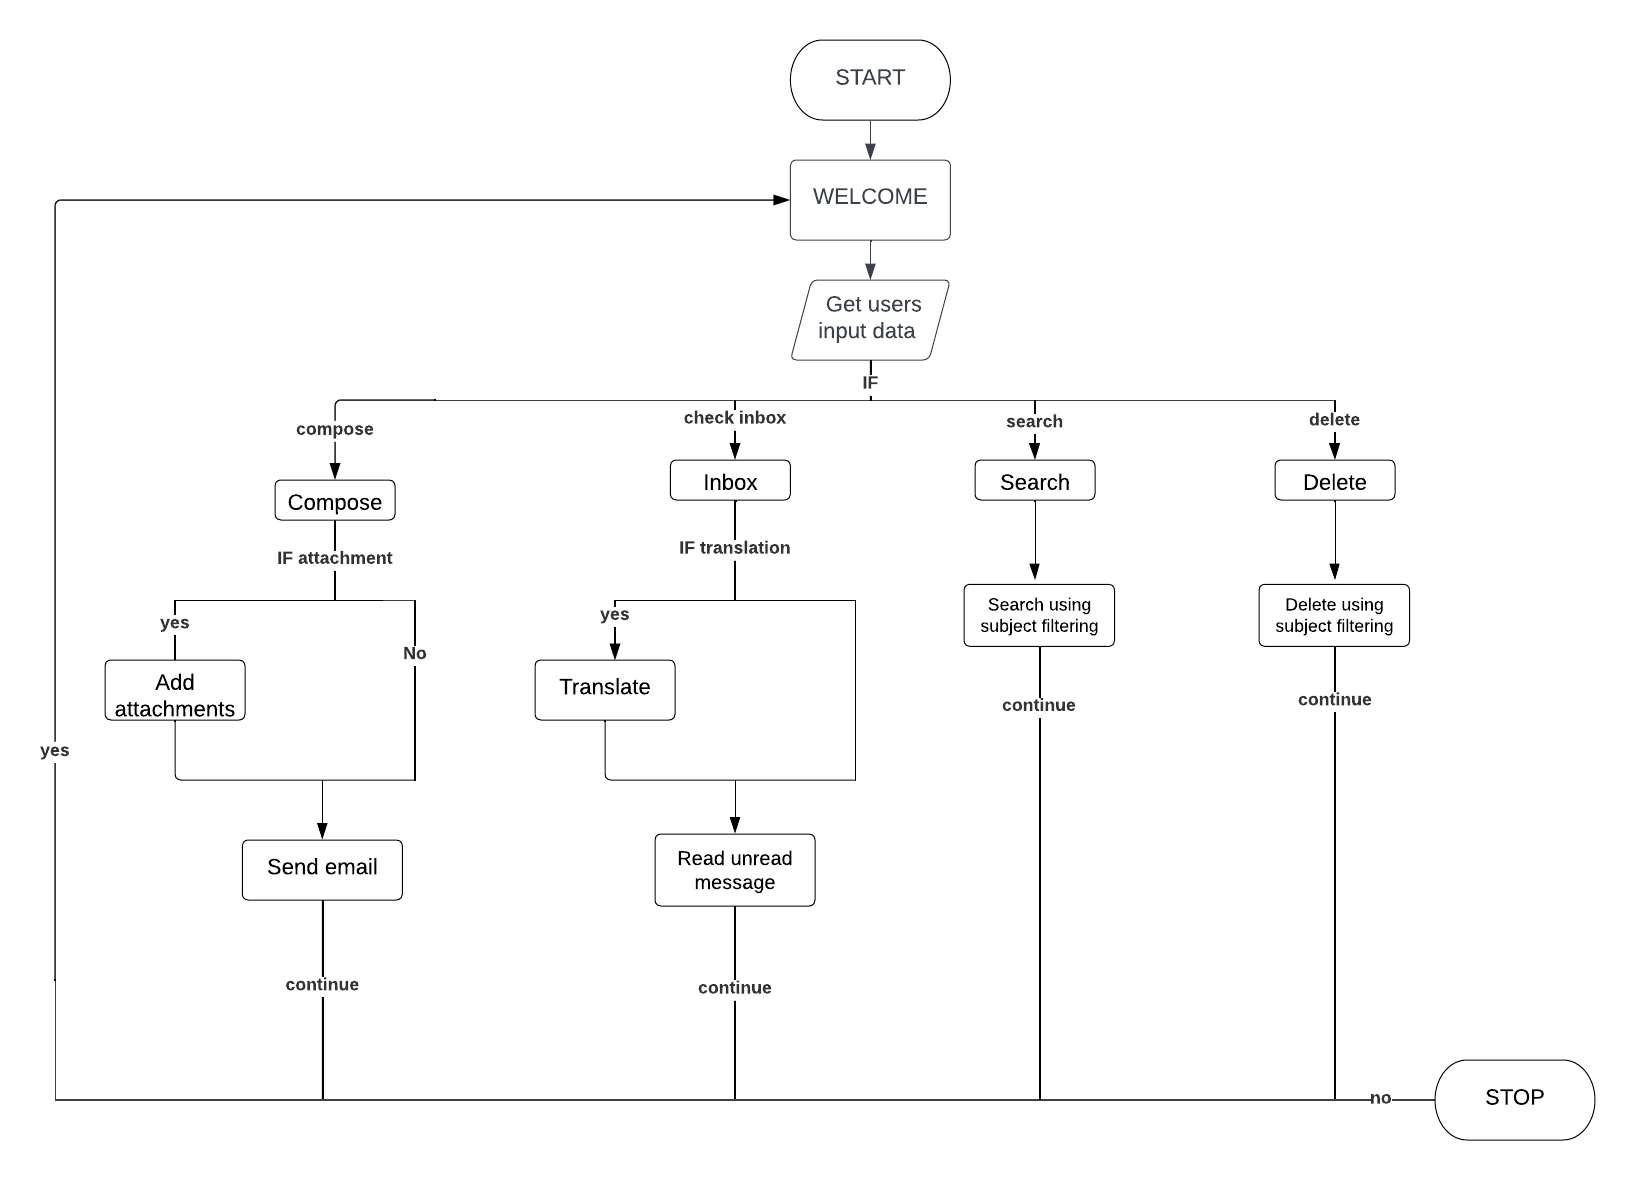
\includegraphics[scale=0.60]{5.png}
  \caption{Workflow} 

   \label{fig:is}
\end{center}
\end{figure}

\newpage

% Section 4 of Chapter 3
\section{Implementation}
The implementation of the proposed voice-based email system for visually impaired individuals involves several steps. Firstly, the system requires a microphone for the user to input voice commands. These voice commands are then processed through a speech-to-text system, which uses the Python programming language to convert the spoken words into text. The text is then used to execute various email functions such as sending, receiving, and composing emails. Once the email function is performed, the system uses a text-to-speech system to read the email content back to the user in their regional language of Malayalam. This provides better understanding and accessibility for visually impaired individuals.\newline \newline
In addition to the basic email functionalities, the system also includes voice-based assistants to guide the user through the email process. This includes step-by-step instructions on how to perform various functions such as composing an email or sending a reply. The system also provides an option to save and store email addresses and contacts for future use. This eliminates the need for the user to remember the email addresses or type them in each time they wish to send an email.\newline \newline
The use of the Malayalam language for the text-to-speech function makes the system more accessible and user-friendly for visually impaired individuals in Kerala, India. This is especially important as Malayalam is the official language of Kerala and is widely spoken by its residents. The implementation of this feature not only makes the system more accessible but also helps promote inclusivity and equal access to technology for visually impaired individuals in the region.



% Chapter 4
\chapter{Agile Methodology}

% Section 1 of Chapter 4
\section{Introduction}
Agile methodology is a popular approach to software development that is well-suited for the development of a voice-based email system for visually impaired people. Agile methodology is an iterative and incremental approach to software development that focuses on delivering working software quickly and continuously improving it over time. It is based on the principles of collaboration, flexibility, and rapid feedback. Agile methodology is particularly useful for software development projects that involve a high level of complexity and uncertainty, such as the development of the voice-based email system.\newline \newline
The agile methodology consists of several key practices that are designed to promote collaboration, rapid feedback, and continuous improvement. The first key practice is iterative development, which involves breaking the development process into small, manageable pieces or iterations. Each iteration involves a short period of time, typically one to four weeks, during which the development team works to complete a specific set of tasks or deliverables. At the end of each iteration, the team reviews the work completed and adjusts the development plan as necessary.\newline \newline
The second key practice is continuous integration, which involves integrating the work of different developers into a single, unified code base on a regular basis. This helps to ensure that the code is always up-to-date and that any issues or conflicts are identified and resolved quickly. The third key practice is test-driven development, which involves writing automated tests for each new piece of code before it is integrated into the code base. This helps to ensure that the code is of high quality and that any defects are identified and corrected quickly.\newline \newline
In the case of the voice-based email system, the agile methodology can be particularly useful in ensuring that the system is developed quickly, efficiently, and in a manner that is responsive to the needs of visually impaired users. The iterative development approach can be used to break the development process into smaller, more manageable pieces, such as developing individual features or functions of the system. Continuous integration can be used to ensure that the code is always up-to-date and that any issues or conflicts are identified and resolved quickly. Test-driven development can be used to ensure that the system is of high quality and that any defects are identified and corrected quickly. 

% Section 2 of Chapter 4

\section{User Story}

A user story is a concise, high-level description of a feature or functionality of a product that is written from the perspective of the user or customer. It is used to capture the user's needs, goals, and desired outcomes, rather than specifying the technical details of how the feature will be implemented. User stories are a key component of agile software development methodologies, which emphasize collaboration and responding to change over following a rigid plan.\newline \newline
User stories typically follow a simple format, such as "As a [user], I want [goal], so that [benefit]." The user story describes a specific feature or functionality that the user needs in order to achieve a particular goal or outcome. By focusing on the user's needs and goals, user stories help ensure that development efforts are aligned with the user's needs and that the resulting product is more likely to be useful and valuable.\newline \newline
User stories are often written on index cards or sticky notes and can be easily prioritized and organized by the development team. They are used to drive the development process, helping to ensure that the team is building features and functionality that are aligned with the user's needs. As the product evolves and new requirements emerge, user stories can be added, updated, or removed, allowing the team to respond quickly and effectively to changing circumstances. Overall, user stories are an important tool for building better products that meet the needs and goals of the end users. The user story of the system is given in Table 4.1

\begin{table}[htbp]
\centering
\begin{tabular}{ | p {1 cm} | p {2 cm} | p {4 cm} |p {5 cm} | }
\hline
\bfseries User Story ID & \bfseries As a (type of user) & \bfseries I want to & \bfseries So that I can \\
\hline
1 & User & Access email using voice & Stay connected to people \\
\hline
2 & User & Compose mail using voice  & Sent emails without relying on text-based interfaces \\
\hline
3 & User & Sent mail & Receive a confirmation message  \\
\hline
4 & User & Dictate the received mail & Use my voice to Obtain mail  \\
\hline
5 & User & Receive mail in regional language & Understand the mail content clearly  \\
\hline
6 & User & Reply to email & Respond to the received mail  \\
\hline
7 & User & Search & Obtain emails using voice  \\
\hline
8 & User & Detete & Remove emails using voice   \\
\hline
\end{tabular}
\caption{User Story}
\label{tab:mytable}
\end{table}


% Section 3 of Chapter 4

\section{Product Backlog}
The product backlog is a prioritized list of requirements or features that need to be developed for a product. It is a key artifact in agile software development methodologies, such as Scrum, and serves as the single source of truth for all the work that needs to be done on the product.\newline \newline
The product backlog is typically owned by the product owner, who is responsible for prioritizing the items on the backlog based on the needs and goals of the stakeholders. The items on the backlog are typically user stories, which describe the features or functionality of the product from the perspective of the user.\newline \newline
The product backlog is dynamic and evolves over time as new information becomes available or as the product evolves. Items can be added, removed, or reprioritized based on feedback from stakeholders, changes in the market or technology, or other factors. The development team uses the product backlog to plan and execute their work, pulling items from the top of the backlog into each sprint or development cycle. The product backlog of the system is given in Table 4.3 

\begin{table}[htbp]
\begin{center}

\begin{tabular} { | p {0.5 cm} | p {3 cm} | p {3 cm} | p {2 cm} |p {3 cm} | }
 \hline
   \bfseries  ID & \bfseries Name & \bfseries Priority\newline(High/Medium \newline /Low) &  \bfseries Estimate \newline (Hr) & \bfseries Status
(Planned/ \newline Progressing/ Completed)   \\
    \hline
    1 &Voice recognition & High & 75 & Completed \\  \hline
    2 &Email configuration & High & 30 & Completed \\  \hline
    3 &Email composition & High & 40 & Completed \\  \hline
    4 &Email delete & High & 40 & Completed \\  \hline
    
    5 & Email reading & High & 65 & Completed \\  \hline
    6 & Reply email & Medium & 24 & Completed \\  \hline
    7 & Language translation & High & 50 & Completed \\  \hline

\end{tabular}
\caption{Product Backlog}
\label{tab:mytable}
\end{center}
\end{table}

% Section 4 of Chapter 4
\section{Project Plan}

A project plan is a detailed document that outlines the objectives, tasks, timelines, resources, and potential risks associated with a specific project. It serves as a roadmap that guides the project team in executing and completing the project successfully within the defined constraints, such as budget, timeline, and scope. \newline \newline
A project plan is critical for ensuring that a project is completed efficiently, effectively, and on time. It helps project managers and team members stay focused on the project goals and objectives and provides a framework for managing tasks, timelines, and resources. A well-defined project plan also helps identify potential risks and challenges, allowing project teams to prepare and implement appropriate strategies to mitigate them. Ultimately, a project plan is essential for managing a project and ensuring that it meets or exceeds stakeholders' expectations.The product plan of the system is given in Table 4.4
\begin{table}[htbp]
\centering
\begin{tblr}{
  cell{2}{2} = {r=2}{},
  cell{4}{2} = {r=2}{},
  cell{6}{2} = {r=2}{},
  cell{8}{2} = {r=2}{},
  vlines,
  hline{1-2,4,6,8,10} = {-}{},
  hline{3,5,7,9} = {1,3-6}{},
}
{\textbf{User }\\\textbf{Story }\\\textbf{ID}}& \textbf{Task Name} & \textbf{Start Date} & \textbf{End Date} &\textbf{Days} & \textbf{Status}  \\
1 & Sprint 1 & 01/02/2023 & 10/02/2023 & 10 & Completed  \\
2 & Sprint 1 & 11/02/2023 & 21/02/2023 & 11 & Completed  \\
3 &Sprint 2 & 27/07/2023 & 08/03/2023 & 10 & Completed \\
4 & Sprint 2 & 09/03/2023 & 20/03/2023 & 11 & Completed \\
5 & Sprint 3 & 22/03/2023 & 31/03/2023 & 10 & Completed \\
6 & Sprint 3 & 01/04/2023 & 11/04/2023 & 11& Completed \\
7 & Sprint 4 & 15/04/2023 & 24/04/2023 & 10  & Completed \\
8 & Sprint 4 & 25/04/2023 & 05/05/2023 & 11 & Completed \\
\end{tblr}
\caption{Project Plan}
\label{tab:mytable}
\end{table}




% Section 5 of Chapter 4
\section{Sprint Backlog (Plan)}
The Sprint Backlog is a plan created by the Development Team at the beginning of each Sprint. It details the work that needs to be completed during the Sprint to meet the Sprint Goal. The Sprint Backlog is created during the Sprint Planning event, where the Development Team decides on the work that will be completed during the Sprint. The Product Owner presents the Product Backlog items that they want to be completed during the Sprint, and the Development Team determines how much of the work they can realistically complete during the Sprint. The detailed sprint backlog (Plan) is given below.
\begin{table}[htbp]
\LARGE
\resizebox{\textwidth}{!}{%
\begin{tblr}{
  vline{1-14} = {1-5}{},
  vline{-} = {7-12}{},
  hline{1-6} = {1-13}{},
  hline{7-13} = {-}{},
}
{\textbf{Backlog}\\\textbf{item}}    & {\textbf{Completion~}\\\textbf{date}} & {\textbf{Original~}\\\textbf{estimate~}} & {\textbf{Day 1}\\\textbf{01/02/2023}}  & {\textbf{Day 2}\\\textbf{02/02/2023}}  & {\textbf{Day 3}\\\textbf{03/02/2023}}  & {\textbf{Day4}\\\textbf{04/02/2023}}   & {\textbf{Day 5}\\\textbf{05/02/2023}}  & {\textbf{Day 6}\\\textbf{06/02/2023}}  & {\textbf{Day 7}\\\textbf{07/02/2023}}  & {\textbf{Day 8}\\\textbf{08/02/2023}}  & {\textbf{Day 9}\\\textbf{09/02/2023}}  & {\textbf{Day 10}\\\textbf{10/02/2023}} &                                   \\
{\textbf{User~}\\\textbf{Story \#1}} &                                       & \textbf{Hours}                           & \textbf{\textbf{Hours}}           & \textbf{\textbf{Hours}}           & \textbf{\textbf{Hours}}           & \textbf{\textbf{Hours}}           & \textbf{\textbf{Hours}}           & \textbf{\textbf{Hours}}           & \textbf{\textbf{Hours}}           & \textbf{\textbf{Hours}}           & \textbf{\textbf{Hours}}           & \textbf{\textbf{Hours}}           &                                   \\
{\textbf{Form }\\\textbf{Design}}    & 10/02/2023                              & 3                                        & 0                                 & 0                                 & 0                                 & 0                                 & 0                                 & 0                                 & 0                                 & 1                                 & 1                                 & 1                                 &                                   \\
\textbf{Coding}                      & 05/02/2023                              & 5                                        & 1                                 & 1                                 & 1                                 & 1                                 & 1                                 & 0                                 & 0                                 & 0                                 & 0                                 & 0                                 &                                   \\
\textbf{Testing}                     & 07/02/2023                              & 2                                        & 0                                 & 0                                 & 0                                 & 0                                 & 0                                 & 1                                 & 1                                 & 0                                 & 0                                 & 0                                 &                                   \\
                                     &                                       &                                          &                                   &                                   &                                   &                                   &                                   &                                   &                                   &                                   &                                   &                                   &                                   \\
{\textbf{Backlog }\\\textbf{item}}   & {\textbf{Completion}\\\textbf{date}}  & {\textbf{Original~}\\\textbf{estimate}}  & {\textbf{Day 11}\\\textbf{11/02/2023}} & {\textbf{Day 12}\\\textbf{12/02/2023}} & {\textbf{Day 13}\\\textbf{13/02/2023}} & {\textbf{Day 14}\\\textbf{14/02/2023}} & {\textbf{Day 15}\\\textbf{15/02/2023}} & {\textbf{Day 16}\\\textbf{16/02/2023}} & {\textbf{Day 17}\\\textbf{17/02/2023}} & {\textbf{Day 18}\\\textbf{18/02/2023}} & {\textbf{Day 19}\\\textbf{19/02/2023}} & {\textbf{Day 20/2023}\\\textbf{20/02/2023}} & {\textbf{Day 21}\\\textbf{21/02/2023}} \\
{\textbf{User~}\\\textbf{Story \#2}} &                                       & \textbf{\textbf{Hours}}                  & \textbf{\textbf{Hours}}           & \textbf{\textbf{Hours}}           & \textbf{\textbf{Hours}}           & \textbf{\textbf{Hours}}           & \textbf{\textbf{Hours}}           & \textbf{\textbf{Hours}}           & \textbf{\textbf{Hours}}           & \textbf{\textbf{Hours}}           & \textbf{\textbf{Hours}}           & \textbf{\textbf{Hours}}           & \textbf{\textbf{Hours}}           \\
{\textbf{Form}\\\textbf{Design}}     & 21/02/2023                              & 3                                        & 0                                 & 0                                 & 0                                 & 0                                 & 0                                 & 0                                 & 0                                 & 0                                 & 1                                 & 1                                 & 1                                 \\
\textbf{Coding}                      & 12/02/2023                              & 6                                        & 1                                 & 1                                 & 1                                 & 1                                 & 1                                 & 1                                 & 0                                 & 0                                 & 0                                 & 0                                 & 0                                 \\
\textbf{Testing}                     & 18/0220/23                              & 2                                        & 0                                 & 0                                 & 0                                 & 0                                 & 0                                 & 0                                 & 1                                 & 1                                 & 0                                 & 0                                 & 0                                 \\
\textbf{Total}                       &                                       & 21                                       &2                                   &1                                   & 2                                  &1                                   &2                                   &2                                   &4                                   &1                                   &3                                 &2                                   &1                                   
\end{tblr}
}
\caption{Sprint Backlog (Plan) - Sprint 1 }
\label{tab:mytable}
\end{table}


\begin{table}[htbp]
\LARGE
\resizebox{\textwidth}{!}{%
\begin{tblr}{
  vline{1-14} = {1-5}{},
  vline{-} = {7-12}{},
  hline{1-6} = {1-13}{},
  hline{7-13} = {-}{},
}
{\textbf{Backlog}\\\textbf{item}}    & {\textbf{Completion~}\\\textbf{date}} & {\textbf{Original~}\\\textbf{estimate~}} & {\textbf{Day 1}\\\textbf{27/02/2023}}           & {\textbf{Day 2}\\\textbf{28/02\textbf{/2023}}}  & {\textbf{Day 3}\\\textbf{01/03\textbf{/2023}}}  & {\textbf{Day4}\\\textbf{02/02\textbf{/2023}}}   & {\textbf{Day 5}\\\textbf{03/03\textbf{/2023}}}  & {\textbf{Day 6}\\\textbf{04/03\textbf{/2023}}}  & {\textbf{Day 7}\\\textbf{05/03\textbf{/2023}}}  & {\textbf{Day 8}\\\textbf{06/03\textbf{/2023}}}  & {\textbf{Day 9}\\\textbf{07/03\textbf{/2023}}}  & {\textbf{Day 10}\\\textbf{08/03\textbf{/2023}}} &                                                 \\
{\textbf{User~}\\\textbf{Story \#3}} &                                       & \textbf{Hours}                           & \textbf{\textbf{Hours}}                         & \textbf{\textbf{Hours}}                         & \textbf{\textbf{Hours}}                         & \textbf{\textbf{Hours}}                         & \textbf{\textbf{Hours}}                         & \textbf{\textbf{Hours}}                         & \textbf{\textbf{Hours}}                         & \textbf{\textbf{Hours}}                         & \textbf{\textbf{Hours}}                         & \textbf{\textbf{Hours}}                         &                                                 \\
{\textbf{Form }\\\textbf{Design}}    & 08/03/2023                            & 3                                        & 0                                               & 0                                               & 0                                               & 0                                               & 0                                               & 0                                               & 0                                               & 1                                               & 1                                               & 1                                               &                                                 \\
\textbf{Coding}                      & 03/03/2023                            & 5                                        & 1                                               & 1                                               & 1                                               & 1                                               & 1                                               & 0                                               & 0                                               & 0                                               & 0                                               & 0                                               &                                                 \\
\textbf{Testing}                     & 05/03/2023                            & 2                                        & 0                                               & 0                                               & 0                                               & 0                                               & 0                                               & 1                                               & 1                                               & 0                                               & 0                                               & 0                                               &                                                 \\
                                     &                                       &                                          &                                                 &                                                 &                                                 &                                                 &                                                 &                                                 &                                                 &                                                 &                                                 &                                                 &                                                 \\
{\textbf{Backlog }\\\textbf{item}}   & {\textbf{Completion}\\\textbf{date}}  & {\textbf{Original~}\\\textbf{estimate}}  & {\textbf{Day 11}\\\textbf{09/03\textbf{/2023}}} & {\textbf{Day 12}\\\textbf{10/03\textbf{/2023}}} & {\textbf{Day 13}\\\textbf{11/03\textbf{/2023}}} & {\textbf{Day 14}\\\textbf{12/03\textbf{/2023}}} & {\textbf{Day 15}\\\textbf{13/03\textbf{/2023}}} & {\textbf{Day 16}\\\textbf{14/03\textbf{/2023}}} & {\textbf{Day 17}\\\textbf{15/03\textbf{/2023}}} & {\textbf{Day 18}\\\textbf{16/03\textbf{/2023}}} & {\textbf{Day 19}\\\textbf{17/03\textbf{/2023}}} & {\textbf{Day 20}\\\textbf{18/03\textbf{/2023}}} & {\textbf{Day 21}\\\textbf{19/03\textbf{/2023}}} \\
{\textbf{User~}\\\textbf{Story \#4}} &                                       & \textbf{\textbf{Hours}}                  & \textbf{\textbf{Hours}}                         & \textbf{\textbf{Hours}}                         & \textbf{\textbf{Hours}}                         & \textbf{\textbf{Hours}}                         & \textbf{\textbf{Hours}}                         & \textbf{\textbf{Hours}}                         & \textbf{\textbf{Hours}}                         & \textbf{\textbf{Hours}}                         & \textbf{\textbf{Hours}}                         & \textbf{\textbf{Hours}}                         & \textbf{\textbf{Hours}}                         \\
{\textbf{Form}\\\textbf{Design}}     & 19/03/2023                            & 3                                        & 0                                               & 0                                               & 0                                               & 0                                               & 0                                               & 0                                               & 0                                               & 0                                               & 1                                               & 1                                               & 1                                               \\
\textbf{Coding}                      & 13/03/2023                            & 6                                        & 1                                               & 1                                               & 1                                               & 1                                               & 1                                               & 1                                               & 0                                               & 0                                               & 0                                               & 0                                               & 0                                               \\
\textbf{Testing}                     & 16/03/2023                            & 2                                        & 0                                               & 0                                               & 0                                               & 0                                               & 0                                               & 0                                               & 1                                               & 1                                               & 0                                               & 0                                               & 0                                               \\
\textbf{Total}                       &                                       & 21                                       &2                                                 &2                                                 & 2                                                &2                                                 &1                                                 &3                                                 &2                                                 &2                                                 &2                                                 &2                                                 &1                                                 
\end{tblr}
}
\caption{Sprint Backlog (Plan) - Sprint 2 }
\label{tab:mytable}

\end{table}

\begin{table}[htbp]
\LARGE
\resizebox{\textwidth}{!}{%
\begin{tblr}{
  vline{1-14} = {1-5}{},
  vline{-} = {7-12}{},
  hline{1-6} = {1-13}{},
  hline{7-13} = {-}{},
}
{\textbf{Backlog}\\\textbf{item}}    & {\textbf{Completion~}\\\textbf{date}} & {\textbf{Original~}\\\textbf{estimate~}} & {\textbf{Day 1}\\\textbf{22/03/2023}}           & {\textbf{Day 2}\\\textbf{23/03\textbf{/2023}}}  & {\textbf{Day 3}\\\textbf{24/03\textbf{/2023}}}  & {\textbf{Day4}\\\textbf{25/02\textbf{/2023}}}   & {\textbf{Day 5}\\\textbf{26/03\textbf{/2023}}}  & {\textbf{Day 6}\\\textbf{27/03\textbf{/2023}}}  & {\textbf{Day 7}\\\textbf{28/03\textbf{/2023}}}  & {\textbf{Day 8}\\\textbf{29/03\textbf{/2023}}}  & {\textbf{Day 9}\\\textbf{30/03\textbf{/2023}}}  & {\textbf{Day 10}\\\textbf{31/03\textbf{/2023}}} &                                                 \\
{\textbf{User~}\\\textbf{Story \#5}} &                                       & \textbf{Hours}                           & \textbf{\textbf{Hours}}                         & \textbf{\textbf{Hours}}                         & \textbf{\textbf{Hours}}                         & \textbf{\textbf{Hours}}                         & \textbf{\textbf{Hours}}                         & \textbf{\textbf{Hours}}                         & \textbf{\textbf{Hours}}                         & \textbf{\textbf{Hours}}                         & \textbf{\textbf{Hours}}                         & \textbf{\textbf{Hours}}                         &                                                 \\
{\textbf{Form }\\\textbf{Design}}    & 31/03/2023                            & 3                                        & 0                                               & 0                                               & 0                                               & 0                                               & 0                                               & 0                                               & 0                                               & 1                                               & 1                                               & 1                                               &                                                 \\
\textbf{Coding}                      & 26/03/2023                            & 5                                        & 1                                               & 1                                               & 1                                               & 1                                               & 1                                               & 0                                               & 0                                               & 0                                               & 0                                               & 0                                               &                                                 \\
\textbf{Testing}                     & 28/03/2023                            & 2                                        & 0                                               & 0                                               & 0                                               & 0                                               & 0                                               & 1                                               & 1                                               & 0                                               & 0                                               & 0                                               &                                                 \\
                                     &                                       &                                          &                                                 &                                                 &                                                 &                                                 &                                                 &                                                 &                                                 &                                                 &                                                 &                                                 &                                                 \\
{\textbf{Backlog }\\\textbf{item}}   & {\textbf{Completion}\\\textbf{date}}  & {\textbf{Original~}\\\textbf{estimate}}  & {\textbf{Day 11}\\\textbf{01/04\textbf{/2023}}} & {\textbf{Day 12}\\\textbf{02/04\textbf{/2023}}} & {\textbf{Day 13}\\\textbf{03/04\textbf{/2023}}} & {\textbf{Day 14}\\\textbf{04/04\textbf{/2023}}} & {\textbf{Day 15}\\\textbf{05/04\textbf{/2023}}} & {\textbf{Day 16}\\\textbf{06/04\textbf{/2023}}} & {\textbf{Day 17}\\\textbf{07/04\textbf{/2023}}} & {\textbf{Day 18}\\\textbf{08/04\textbf{/2023}}} & {\textbf{Day 19}\\\textbf{09/04\textbf{/2023}}} & {\textbf{Day 20}\\\textbf{10/04\textbf{/2023}}} & {\textbf{Day 21}\\\textbf{11/04\textbf{/2023}}} \\
{\textbf{User~}\\\textbf{Story \#6}} &                                       & \textbf{\textbf{Hours}}                  & \textbf{\textbf{Hours}}                         & \textbf{\textbf{Hours}}                         & \textbf{\textbf{Hours}}                         & \textbf{\textbf{Hours}}                         & \textbf{\textbf{Hours}}                         & \textbf{\textbf{Hours}}                         & \textbf{\textbf{Hours}}                         & \textbf{\textbf{Hours}}                         & \textbf{\textbf{Hours}}                         & \textbf{\textbf{Hours}}                         & \textbf{\textbf{Hours}}                         \\
{\textbf{Form}\\\textbf{Design}}     & 11/04/2023                            & 3                                        & 0                                               & 0                                               & 0                                               & 0                                               & 0                                               & 0                                               & 0                                               & 0                                               & 1                                               & 1                                               & 1                                               \\
\textbf{Coding}                      & 06/04/2023                            & 6                                        & 1                                               & 1                                               & 1                                               & 1                                               & 1                                               & 1                                               & 0                                               & 0                                               & 0                                               & 0                                               & 0                                               \\
\textbf{Testing}                     & 08/04/2023                            & 2                                        & 0                                               & 0                                               & 0                                               & 0                                               & 0                                               & 0                                               & 1                                               & 1                                               & 0                                               & 0                                               & 0                                               \\
\textbf{Total}                       &                                       & 21                                       &2                                                 &2                                                 &1                                                 & 2                                                &2                                                 &3                                                 &2                                                 &2                                                 &2                                                 &2                                                 & 1                                                
\end{tblr}
}
\caption{Sprint Backlog (Plan) - Sprint 3 }
\label{tab:mytable}
\end{table}
\begin{table}[htbp]
\LARGE
\resizebox{\textwidth}{!}{%
\begin{tblr}{
  vline{1-14} = {1-5}{},
  vline{-} = {7-12}{},
  hline{1-6} = {1-13}{},
  hline{7-13} = {-}{},
}
{\textbf{Backlog}\\\textbf{item}}    & {\textbf{Completion~}\\\textbf{date}} & {\textbf{Original~}\\\textbf{estimate~}} & {\textbf{Day 1}\\\textbf{15/04/2023}}           & {\textbf{Day 2}\\\textbf{16/04\textbf{/2023}}}  & {\textbf{Day 3}\\\textbf{17/04\textbf{/2023}}}  & {\textbf{Day4}\\\textbf{18/04\textbf{/2023}}}   & {\textbf{Day 5}\\\textbf{19/04\textbf{/2023}}}  & {\textbf{Day 6}\\\textbf{20/04\textbf{/2023}}}  & {\textbf{Day 7}\\\textbf{21/04\textbf{/2023}}}  & {\textbf{Day 8}\\\textbf{22/04\textbf{/2023}}}  & {\textbf{Day 9}\\\textbf{23/04\textbf{/2023}}}  & {\textbf{Day 10}\\\textbf{24/04\textbf{/2023}}} &                                                 \\
{\textbf{User~}\\\textbf{Story \#7}} &                                       & \textbf{Hours}                           & \textbf{\textbf{Hours}}                         & \textbf{\textbf{Hours}}                         & \textbf{\textbf{Hours}}                         & \textbf{\textbf{Hours}}                         & \textbf{\textbf{Hours}}                         & \textbf{\textbf{Hours}}                         & \textbf{\textbf{Hours}}                         & \textbf{\textbf{Hours}}                         & \textbf{\textbf{Hours}}                         & \textbf{\textbf{Hours}}                         &                                                 \\
{\textbf{Form }\\\textbf{Design}}    & 24/04/2023                            & 3                                        & 0                                               & 0                                               & 0                                               & 0                                               & 0                                               & 0                                               & 0                                               & 1                                               & 1                                               & 1                                               &                                                 \\
\textbf{Coding}                      & 19/04/2023                            & 5                                        & 1                                               & 1                                               & 1                                               & 1                                               & 1                                               & 0                                               & 0                                               & 0                                               & 0                                               & 0                                               &                                                 \\
\textbf{Testing}                     & 21/04/2023                            & 2                                        & 0                                               & 0                                               & 0                                               & 0                                               & 0                                               & 1                                               & 1                                               & 0                                               & 0                                               & 0                                               &                                                 \\
                                     &                                       &                                          &                                                 &                                                 &                                                 &                                                 &                                                 &                                                 &                                                 &                                                 &                                                 &                                                 &                                                 \\
{\textbf{Backlog }\\\textbf{item}}   & {\textbf{Completion}\\\textbf{date}}  & {\textbf{Original~}\\\textbf{estimate}}  & {\textbf{Day 11}\\\textbf{25/04\textbf{/2023}}} & {\textbf{Day 12}\\\textbf{26/04\textbf{/2023}}} & {\textbf{Day 13}\\\textbf{27/04\textbf{/2023}}} & {\textbf{Day 14}\\\textbf{28/04\textbf{/2023}}} & {\textbf{Day 15}\\\textbf{29/04\textbf{/2023}}} & {\textbf{Day 16}\\\textbf{30/04\textbf{/2023}}} & {\textbf{Day 17}\\\textbf{01/05\textbf{/2023}}} & {\textbf{Day 18}\\\textbf{02/05\textbf{/2023}}} & {\textbf{Day 19}\\\textbf{03/05\textbf{/2023}}} & {\textbf{Day 20}\\\textbf{04/05\textbf{/2023}}} & {\textbf{Day 21}\\\textbf{05/05\textbf{/2023}}} \\
{\textbf{User~}\\\textbf{Story \#8}} &                                       & \textbf{\textbf{Hours}}                  & \textbf{\textbf{Hours}}                         & \textbf{\textbf{Hours}}                         & \textbf{\textbf{Hours}}                         & \textbf{\textbf{Hours}}                         & \textbf{\textbf{Hours}}                         & \textbf{\textbf{Hours}}                         & \textbf{\textbf{Hours}}                         & \textbf{\textbf{Hours}}                         & \textbf{\textbf{Hours}}                         & \textbf{\textbf{Hours}}                         & \textbf{\textbf{Hours}}                         \\
{\textbf{Form}\\\textbf{Design}}     & 05/05/2023                            & 3                                        & 0                                               & 0                                               & 0                                               & 0                                               & 0                                               & 0                                               & 0                                               & 0                                               & 1                                               & 1                                               & 1                                               \\
\textbf{Coding}                      & 30/04/2023                            & 6                                        & 1                                               & 1                                               & 1                                               & 1                                               & 1                                               & 1                                               & 0                                               & 0                                               & 0                                               & 0                                               & 0                                               \\
\textbf{Testing}                     & 02/05/2023                            & 2                                        & 0                                               & 0                                               & 0                                               & 0                                               & 0                                               & 0                                               & 1                                               & 1                                               & 0                                               & 0                                               & 0                                               \\
\textbf{Total}                       &                                       & 21                                       &2                                                 &2                                                 &2                                                 &2                                                 &2                                                 &2                                                 &2                                                 & 2                                                &2                                                 &2                                                 &2                                                 
\end{tblr}
}
\caption{Sprint Backlog (Plan) - Sprint 4 }
\label{tab:mytable}
\end{table}

\newpage
% Section 6 of Chapter 4
\section{Sprint Backlog (Actual)}
The Sprint Backlog is a subset of the Product Backlog, consisting of items that the Development Team has committed to completing during a Sprint. It is created during the Sprint Planning meeting, where the Development Team selects the highest priority Product Backlog items that they can complete within the upcoming Sprint. The Sprint Backlog is a plan for how the Development Team will accomplish the selected Product Backlog items and achieve the Sprint Goal. The detailed sprint backlog (Actual) is given below.
\begin{table}[htbp]
\LARGE
\resizebox{\textwidth}{!}{%
\begin{tblr}{
  vline{1-14} = {1-5}{},
  vline{-} = {7-12}{},
  hline{1-6} = {1-13}{},
  hline{7-13} = {-}{},
}
{\textbf{Backlog}\\\textbf{item}}    & {\textbf{Completion~}\\\textbf{date}} & {\textbf{Original~}\\\textbf{estimate~}} & {\textbf{Day 1}\\\textbf{01/02/2023}}  & {\textbf{Day 2}\\\textbf{02/02/2023}}  & {\textbf{Day 3}\\\textbf{03/02/2023}}  & {\textbf{Day4}\\\textbf{04/02/2023}}   & {\textbf{Day 5}\\\textbf{05/02/2023}}  & {\textbf{Day 6}\\\textbf{06/02/2023}}  & {\textbf{Day 7}\\\textbf{07/02/2023}}  & {\textbf{Day 8}\\\textbf{08/02/2023}}  & {\textbf{Day 9}\\\textbf{09/02/2023}}  & {\textbf{Day 10}\\\textbf{10/02/2023}} &                                   \\
{\textbf{User~}\\\textbf{Story \#1}} &                                       & \textbf{Hours}                           & \textbf{\textbf{Hours}}           & \textbf{\textbf{Hours}}           & \textbf{\textbf{Hours}}           & \textbf{\textbf{Hours}}           & \textbf{\textbf{Hours}}           & \textbf{\textbf{Hours}}           & \textbf{\textbf{Hours}}           & \textbf{\textbf{Hours}}           & \textbf{\textbf{Hours}}           & \textbf{\textbf{Hours}}           &                                   \\
{\textbf{Form }\\\textbf{Design}}    & 10/02/23                              & 3                                        & 0                                 & 0                                 & 0                                 & 0                                 & 0                                 & 0                                 & 0                                 & 1                                 & 1                                 & 1                                 &                                   \\
\textbf{Coding}                      & 08/02/23                              & 5                                        & 1                                 & 0                                & 1                                 & 1                                 & 1                                 & 0                                 & 1                                 & 0                                 & 0                                 & 0                                 &                                   \\
\textbf{Testing}                     & 07/02/23                              & 2                                        & 0                                 & 0                                 & 0                                 & 0                                 & 0                                 & 1                                 & 1                                 & 0                                 & 0                                 & 0                                 &                                   \\
                                     &                                       &                                          &                                   &                                   &                                   &                                   &                                   &                                   &                                   &                                   &                                   &                                   &                                   \\
{\textbf{Backlog }\\\textbf{item}}   & {\textbf{Completion}\\\textbf{date}}  & {\textbf{Original~}\\\textbf{estimate}}  & {\textbf{Day 11}\\\textbf{11/02/2023}} & {\textbf{Day 12}\\\textbf{12/02/2023}} & {\textbf{Day 13}\\\textbf{13/02/2023}} & {\textbf{Day 14}\\\textbf{14/02/2023}} & {\textbf{Day 15}\\\textbf{15/02/2023}} & {\textbf{Day 16}\\\textbf{16/02/2023}} & {\textbf{Day 17}\\\textbf{17/02/2023}} & {\textbf{Day 18}\\\textbf{18/02/2023}} & {\textbf{Day 19}\\\textbf{19/02/2023}} & {\textbf{Day 20/2023}\\\textbf{20/02/2023}} & {\textbf{Day 21}\\\textbf{21/02/2023}} \\
{\textbf{User~}\\\textbf{Story \#2}} &                                       & \textbf{\textbf{Hours}}                  & \textbf{\textbf{Hours}}           & \textbf{\textbf{Hours}}           & \textbf{\textbf{Hours}}           & \textbf{\textbf{Hours}}           & \textbf{\textbf{Hours}}           & \textbf{\textbf{Hours}}           & \textbf{\textbf{Hours}}           & \textbf{\textbf{Hours}}           & \textbf{\textbf{Hours}}           & \textbf{\textbf{Hours}}           & \textbf{\textbf{Hours}}           \\
{\textbf{Form}\\\textbf{Design}}     & 21/02/23                              & 3                                        & 0                                 & 0                                 & 0                                 & 0                                 & 0                                 & 0                                 & 0                                 & 0                                 & 1                                 & 1                                 & 1                                 \\
\textbf{Coding}                      & 13/02/23                              & 6                                        & 1                                 & 1                                 & 1                                 & 0                                 & 1                                 & 1                                 & 1                                 & 0                                 & 0                                 & 0                                 & 0                                 \\
\textbf{Testing}                     & 19/02/23                              & 2                                        & 0                                 & 0                                 & 0                                 & 0                                 & 0                                 & 0                                 & 1                                 & 0                                 & 1                                 & 0                                 & 0                                 \\
\textbf{Total}                       &                                       & 21                                       & 2                                  & 1                                  &2                                   &1                                   & 2                                  &2                                   &4                                   & 1                                  &3                                   &2                                   & 1                                  
\end{tblr}
}
\caption{Sprint Backlog (Actual) - Sprint 1 }
\label{tab:mytable}
\end{table}

\begin{table}[htbp]
\LARGE
\resizebox{\textwidth}{!}{%
\begin{tblr}{
  vline{1-14} = {1-5}{},
  vline{-} = {7-12}{},
  hline{1-6} = {1-13}{},
  hline{7-13} = {-}{},
}
{\textbf{Backlog}\\\textbf{item}}    & {\textbf{Completion~}\\\textbf{date}} & {\textbf{Original~}\\\textbf{estimate~}} & {\textbf{Day 1}\\\textbf{27/02/2023}}           & {\textbf{Day 2}\\\textbf{28/02\textbf{/2023}}}  & {\textbf{Day 3}\\\textbf{01/03\textbf{/2023}}}  & {\textbf{Day4}\\\textbf{02/02\textbf{/2023}}}   & {\textbf{Day 5}\\\textbf{03/03\textbf{/2023}}}  & {\textbf{Day 6}\\\textbf{04/03\textbf{/2023}}}  & {\textbf{Day 7}\\\textbf{05/03\textbf{/2023}}}  & {\textbf{Day 8}\\\textbf{06/03\textbf{/2023}}}  & {\textbf{Day 9}\\\textbf{07/03\textbf{/2023}}}  & {\textbf{Day 10}\\\textbf{08/03\textbf{/2023}}} &                                                 \\
{\textbf{User~}\\\textbf{Story \#3}} &                                       & \textbf{Hours}                           & \textbf{\textbf{Hours}}                         & \textbf{\textbf{Hours}}                         & \textbf{\textbf{Hours}}                         & \textbf{\textbf{Hours}}                         & \textbf{\textbf{Hours}}                         & \textbf{\textbf{Hours}}                         & \textbf{\textbf{Hours}}                         & \textbf{\textbf{Hours}}                         & \textbf{\textbf{Hours}}                         & \textbf{\textbf{Hours}}                         &                                                 \\
{\textbf{Form }\\\textbf{Design}}    & 08/03/2023                            & 3                                        & 0                                               & 0                                               & 0                                               & 0                                               & 0                                               & 0                                               & 0                                               & 1                                               & 1                                               & 1                                               &                                                 \\
\textbf{Coding}                      & 04/03/2023                            & 5                                        & 1                                               & 1                                               & 1                                               & 1                                               & 0                                               & 1                                               & 0                                               & 0                                               & 0                                               & 0                                               &                                                 \\
\textbf{Testing}                     & 05/03/2023                            & 2                                        & 0                                               & 0                                               & 0                                               & 0                                               & 0                                               & 1                                               & 1                                               & 0                                               & 0                                               & 0                                               &                                                 \\
                                     &                                       &                                          &                                                 &                                                 &                                                 &                                                 &                                                 &                                                 &                                                 &                                                 &                                                 &                                                 &                                                 \\
{\textbf{Backlog }\\\textbf{item}}   & {\textbf{Completion}\\\textbf{date}}  & {\textbf{Original~}\\\textbf{estimate}}  & {\textbf{Day 11}\\\textbf{09/03\textbf{/2023}}} & {\textbf{Day 12}\\\textbf{10/03\textbf{/2023}}} & {\textbf{Day 13}\\\textbf{11/03\textbf{/2023}}} & {\textbf{Day 14}\\\textbf{12/03\textbf{/2023}}} & {\textbf{Day 15}\\\textbf{13/03\textbf{/2023}}} & {\textbf{Day 16}\\\textbf{14/03\textbf{/2023}}} & {\textbf{Day 17}\\\textbf{15/03\textbf{/2023}}} & {\textbf{Day 18}\\\textbf{16/03\textbf{/2023}}} & {\textbf{Day 19}\\\textbf{17/03\textbf{/2023}}} & {\textbf{Day 20}\\\textbf{18/03\textbf{/2023}}} & {\textbf{Day 21}\\\textbf{19/03\textbf{/2023}}} \\
{\textbf{User~}\\\textbf{Story \#4}} &                                       & \textbf{\textbf{Hours}}                  & \textbf{\textbf{Hours}}                         & \textbf{\textbf{Hours}}                         & \textbf{\textbf{Hours}}                         & \textbf{\textbf{Hours}}                         & \textbf{\textbf{Hours}}                         & \textbf{\textbf{Hours}}                         & \textbf{\textbf{Hours}}                         & \textbf{\textbf{Hours}}                         & \textbf{\textbf{Hours}}                         & \textbf{\textbf{Hours}}                         & \textbf{\textbf{Hours}}                         \\
{\textbf{Form}\\\textbf{Design}}     & 19/03/2023                            & 3                                        & 0                                               & 0                                               & 0                                               & 0                                               & 0                                               & 0                                               & 0                                               & 0                                               & 1                                               & 1                                               & 1                                               \\
\textbf{Coding}                      & 13/03/2023                            & 6                                        & 1                                               & 1                                               & 1                                               & 1                                               & 1                                               & 1                                               & 0                                               & 0                                               & 0                                               & 0                                               & 0                                               \\
\textbf{Testing}                     & 16/03/2023                            & 2                                        & 0                                               & 0                                               & 0                                               & 0                                               & 0                                               & 0                                               & 1                                               & 1                                               & 0                                               & 0                                               & 0                                               \\
\textbf{Total}                       &                                       & 21                                       &  2                                               & 2                                                &   2                                             & 2                                                & 1                                                & 3                                                &2                                                 & 2                                                & 2                                                &2                                                 & 1                                                
\end{tblr}
}
\caption{Sprint Backlog (Actual) - Sprint 2 }
\label{tab:mytable}

\end{table}

% \usepackage{rotating}
% \usepackage{tabularray}
\begin{table}[htbp]
\LARGE
\resizebox{\textwidth}{!}{%
\begin{tblr}{
  vline{1-14} = {1-5}{},
  vline{-} = {7-12}{},
  hline{1-6} = {1-13}{},
  hline{7-13} = {-}{},
}
{\textbf{Backlog}\\\textbf{item}}    & {\textbf{Completion~}\\\textbf{date}} & {\textbf{Original~}\\\textbf{estimate~}} & {\textbf{Day 1}\\\textbf{22/03/2023}}           & {\textbf{Day 2}\\\textbf{23/03\textbf{/2023}}}  & {\textbf{Day 3}\\\textbf{24/03\textbf{/2023}}}  & {\textbf{Day4}\\\textbf{25/02\textbf{/2023}}}   & {\textbf{Day 5}\\\textbf{26/03\textbf{/2023}}}  & {\textbf{Day 6}\\\textbf{27/03\textbf{/2023}}}  & {\textbf{Day 7}\\\textbf{28/03\textbf{/2023}}}  & {\textbf{Day 8}\\\textbf{29/03\textbf{/2023}}}  & {\textbf{Day 9}\\\textbf{30/03\textbf{/2023}}}  & {\textbf{Day 10}\\\textbf{31/03\textbf{/2023}}} &                                                 \\
{\textbf{User~}\\\textbf{Story \#5}} &                                       & \textbf{Hours}                           & \textbf{\textbf{Hours}}                         & \textbf{\textbf{Hours}}                         & \textbf{\textbf{Hours}}                         & \textbf{\textbf{Hours}}                         & \textbf{\textbf{Hours}}                         & \textbf{\textbf{Hours}}                         & \textbf{\textbf{Hours}}                         & \textbf{\textbf{Hours}}                         & \textbf{\textbf{Hours}}                         & \textbf{\textbf{Hours}}                         &                                                 \\
{\textbf{Form }\\\textbf{Design}}    & 31/03/2023                            & 3                                        & 0                                               & 0                                               & 0                                               & 0                                               & 0                                               & 0                                               & 0                                               & 1                                               & 1                                               & 1                                               &                                                 \\
\textbf{Coding}                      & 28/03/2023                            & 5                                        & 1                                               & 1                                               & 0                                               & 1                                               & 1                                               & 0                                               & 1                                               & 0                                               & 0                                               & 0                                               &                                                 \\
\textbf{Testing}                     & 28/03/2023                            & 2                                        & 0                                               & 0                                               & 0                                               & 0                                               & 0                                               & 1                                               & 1                                               & 0                                               & 0                                               & 0                                               &                                                 \\
                                     &                                       &                                          &                                                 &                                                 &                                                 &                                                 &                                                 &                                                 &                                                 &                                                 &                                                 &                                                 &                                                 \\
{\textbf{Backlog }\\\textbf{item}}   & {\textbf{Completion}\\\textbf{date}}  & {\textbf{Original~}\\\textbf{estimate}}  & {\textbf{Day 11}\\\textbf{01/04\textbf{/2023}}} & {\textbf{Day 12}\\\textbf{02/04\textbf{/2023}}} & {\textbf{Day 13}\\\textbf{03/04\textbf{/2023}}} & {\textbf{Day 14}\\\textbf{04/04\textbf{/2023}}} & {\textbf{Day 15}\\\textbf{05/04\textbf{/2023}}} & {\textbf{Day 16}\\\textbf{06/04\textbf{/2023}}} & {\textbf{Day 17}\\\textbf{07/04\textbf{/2023}}} & {\textbf{Day 18}\\\textbf{08/04\textbf{/2023}}} & {\textbf{Day 19}\\\textbf{09/04\textbf{/2023}}} & {\textbf{Day 20}\\\textbf{10/04\textbf{/2023}}} & {\textbf{Day 21}\\\textbf{11/04\textbf{/2023}}} \\
{\textbf{User~}\\\textbf{Story \#6}} &                                       & \textbf{\textbf{Hours}}                  & \textbf{\textbf{Hours}}                         & \textbf{\textbf{Hours}}                         & \textbf{\textbf{Hours}}                         & \textbf{\textbf{Hours}}                         & \textbf{\textbf{Hours}}                         & \textbf{\textbf{Hours}}                         & \textbf{\textbf{Hours}}                         & \textbf{\textbf{Hours}}                         & \textbf{\textbf{Hours}}                         & \textbf{\textbf{Hours}}                         & \textbf{\textbf{Hours}}                         \\
{\textbf{Form}\\\textbf{Design}}     & 11/04/2023                            & 3                                        & 0                                               & 0                                               & 0                                               & 0                                               & 0                                               & 0                                               & 0                                               & 0                                               & 1                                               & 1                                               & 1                                               \\
\textbf{Coding}                      & 06/04/2023                            & 6                                        & 1                                               & 1                                               & 1                                               & 1                                               & 1                                               & 1                                               & 0                                               & 0                                               & 0                                               & 0                                               & 0                                               \\
\textbf{Testing}                     & 08/04/2023                            & 2                                        & 0                                               & 0                                               & 0                                               & 0                                               & 0                                               & 0                                               & 1                                               & 1                                               & 0                                               & 0                                               & 0                                               \\
\textbf{Total}                       &                                       & 21                                       &2                                                 &2                                                 &1                                                 & 2                                                & 2                                                &2                                                 &3                                                 & 2                                                & 2                                                & 2                                                &1                                                 
\end{tblr}
}
\caption{Sprint Backlog (Actual) - Sprint 3 }
\label{tab:mytable}
\end{table}
\begin{table}[htbp]
\LARGE
\resizebox{\textwidth}{!}{%
\begin{tblr}{
  vline{1-14} = {1-5}{},
  vline{-} = {7-12}{},
  hline{1-6} = {1-13}{},
  hline{7-13} = {-}{},
}
{\textbf{Backlog}\\\textbf{item}}    & {\textbf{Completion~}\\\textbf{date}} & {\textbf{Original~}\\\textbf{estimate~}} & {\textbf{Day 1}\\\textbf{15/04/2023}}           & {\textbf{Day 2}\\\textbf{16/04\textbf{/2023}}}  & {\textbf{Day 3}\\\textbf{17/04\textbf{/2023}}}  & {\textbf{Day4}\\\textbf{18/04\textbf{/2023}}}   & {\textbf{Day 5}\\\textbf{19/04\textbf{/2023}}}  & {\textbf{Day 6}\\\textbf{20/04\textbf{/2023}}}  & {\textbf{Day 7}\\\textbf{21/04\textbf{/2023}}}  & {\textbf{Day 8}\\\textbf{22/04\textbf{/2023}}}  & {\textbf{Day 9}\\\textbf{23/04\textbf{/2023}}}  & {\textbf{Day 10}\\\textbf{24/04\textbf{/2023}}} &                                                 \\
{\textbf{User~}\\\textbf{Story \#7}} &                                       & \textbf{Hours}                           & \textbf{\textbf{Hours}}                         & \textbf{\textbf{Hours}}                         & \textbf{\textbf{Hours}}                         & \textbf{\textbf{Hours}}                         & \textbf{\textbf{Hours}}                         & \textbf{\textbf{Hours}}                         & \textbf{\textbf{Hours}}                         & \textbf{\textbf{Hours}}                         & \textbf{\textbf{Hours}}                         & \textbf{\textbf{Hours}}                         &                                                 \\
{\textbf{Form }\\\textbf{Design}}    & 24/04/2023                            & 3                                        & 0                                               & 0                                               & 0                                               & 0                                               & 0                                               & 0                                               & 0                                               & 1                                               & 1                                               & 1                                               &                                                 \\
\textbf{Coding}                      & 19/04/2023                            & 5                                        & 1                                               & 1                                               & 1                                               & 1                                               & 1                                               & 0                                               & 0                                               & 0                                               & 0                                               & 0                                               &                                                 \\
\textbf{Testing}                     & 21/04/2023                            & 2                                        & 0                                               & 0                                               & 0                                               & 0                                               & 0                                               & 1                                               & 1                                               & 0                                               & 0                                               & 0                                               &                                                 \\
                                     &                                       &                                          &                                                 &                                                 &                                                 &                                                 &                                                 &                                                 &                                                 &                                                 &                                                 &                                                 &                                                 \\
{\textbf{Backlog }\\\textbf{item}}   & {\textbf{Completion}\\\textbf{date}}  & {\textbf{Original~}\\\textbf{estimate}}  & {\textbf{Day 11}\\\textbf{25/04\textbf{/2023}}} & {\textbf{Day 12}\\\textbf{26/04\textbf{/2023}}} & {\textbf{Day 13}\\\textbf{27/04\textbf{/2023}}} & {\textbf{Day 14}\\\textbf{28/04\textbf{/2023}}} & {\textbf{Day 15}\\\textbf{29/04\textbf{/2023}}} & {\textbf{Day 16}\\\textbf{30/04\textbf{/2023}}} & {\textbf{Day 17}\\\textbf{01/05\textbf{/2023}}} & {\textbf{Day 18}\\\textbf{02/05\textbf{/2023}}} & {\textbf{Day 19}\\\textbf{03/05\textbf{/2023}}} & {\textbf{Day 20}\\\textbf{04/05\textbf{/2023}}} & {\textbf{Day 21}\\\textbf{05/05\textbf{/2023}}} \\
{\textbf{User~}\\\textbf{Story \#8}} &                                       & \textbf{\textbf{Hours}}                  & \textbf{\textbf{Hours}}                         & \textbf{\textbf{Hours}}                         & \textbf{\textbf{Hours}}                         & \textbf{\textbf{Hours}}                         & \textbf{\textbf{Hours}}                         & \textbf{\textbf{Hours}}                         & \textbf{\textbf{Hours}}                         & \textbf{\textbf{Hours}}                         & \textbf{\textbf{Hours}}                         & \textbf{\textbf{Hours}}                         & \textbf{\textbf{Hours}}                         \\
{\textbf{Form}\\\textbf{Design}}     & 05/05/2023                            & 3                                        & 0                                               & 0                                               & 0                                               & 0                                               & 0                                               & 0                                               & 0                                               & 0                                               & 1                                               & 1                                               & 1                                               \\
\textbf{Coding}                      & 30/04/2023                            & 6                                        & 1                                               & 1                                               & 1                                               & 1                                               & 1                                               & 1                                               & 0                                               & 0                                               & 0                                               & 0                                               & 0                                               \\
\textbf{Testing}                     & 02/05/2023                            & 2                                        & 0                                               & 0                                               & 0                                               & 0                                               & 0                                               & 0                                               & 1                                               & 1                                               & 0                                               & 0                                               & 0                                               \\
\textbf{Total}                       &                                       & 21                                       &2                                                 &2                                                 &  2                                               &2                                               &2                                                 &2                                                 &2                                                 &2                                                 &2                                                 &2                                                 &1                                                 
\end{tblr}
}
\caption{Sprint Backlog (Actual) - Sprint 4 }
\label{tab:mytable}
\end{table}
\newpage
% Section 7 of Chapter 4
\section{Product Backlog Review}
Product Backlog Review is an essential ceremony in Agile software development, where the Product Owner and the Development Team collaborate to review the product backlog items. The primary goal of the Product Backlog Review is to ensure that the product backlog is up-to-date, prioritize the items, and provide a shared understanding of the product backlog among the team. The Product backlog review is given below.
\begin{table}[htbp]
\centering

\begin{tblr}{
  cell{1}{2} = {c},
  cell{2}{2} = {c},
  vline{-} = {3-5}{},
  hline{3-6} = {-}{},
}
                       & \textbf{REVIEW FORM}                                    &                                                          \\
                       & \textbf{SPRINT 1}                                       &                                                          \\
\textbf{User Story ID} & {\textbf{Comments from }\\\textbf{Scrum master if any}} & {\textbf{Comments from}\\\textbf{Product Owner~if any}}  \\
1                      & {Voice recognition accuracy\\could be improved}         & Easy access through voice                                \\
2                      & {Confirm message can be \\added}                        & {Include attachments while sending\\emails if necessary} 
\end{tblr}
\caption{Product Backlog Review - Sprint 1 }
\label{tab:mytable}
\end{table}

\begin{table}[htbp]
\centering
\begin{tblr}{
  cell{1}{2} = {c},
  cell{2}{2} = {c},
  vline{-} = {3-5}{},
  hline{3-6} = {-}{},
}
                       & \textbf{REVIEW FORM}                                    &                                                         \\
                       & \textbf{SPRINT 2}                                       &                                                         \\
\textbf{User Story ID} & {\textbf{Comments from }\\\textbf{Scrum master if any}} & {\textbf{Comments from}\\\textbf{Product Owner~if any}} \\
3                      & Satisfying result                                       & Satisfying result                                       \\
4                      & {Dictate the email in \\Malayalam}                      & {Tell the number of unread \\messages}                  
\end{tblr}

\caption{Product Backlog Review - Sprint 2 }
\label{tab:mytable}
\end{table}

\begin{table}[htbp]
\centering
\begin{tblr}{
  cell{1}{2} = {c},
  cell{2}{2} = {c},
  vline{-} = {3-5}{},
  hline{3-6} = {-}{},
}
                       & \textbf{REVIEW FORM}                                     &                                                           \\
                       & \textbf{SPRINT 3}                                        &                                                           \\
\textbf{User Story ID} & {\textbf{Comments from }\\\textbf{Scrum master if any}}  & {\textbf{Comments from}\\\textbf{Product Owner~if any}}   \\
5                      & {Improve accuracy when \\ converting to regional language} & {Improve accuracy when\\ converting to regional language} \\
6                      & Satisfying result                                        & Satisfying result                                         
\end{tblr}
\caption{Product Backlog Review - Sprint 3 }
\label{tab:mytable}
\end{table}

\begin{table}[htbp]
\centering
\begin{tblr}{
  cell{1}{2} = {c},
  cell{2}{2} = {c},
  vline{-} = {3-5}{},
  hline{3-6} = {-}{},
}
                       & \textbf{REVIEW FORM}                                    &                                                         \\
                       & \textbf{SPRINT 4}                                       &                                                         \\
\textbf{User Story ID} & {\textbf{Comments from }\\\textbf{Scrum master if any}} & {\textbf{Comments from}\\\textbf{Product Owner~if any}} \\
7                      & {Searching can be done using\\a subject filtering}      & Easy search                                             \\
8                      & {Deleting can be done using \\a subject filtering}      & Easy Delete                                             
\end{tblr}
\caption{Product Backlog Review - Sprint 4 }
\label{tab:mytable}
\end{table}


\newpage
% Section 8 of Chapter 4
\section{Sprint Review}
Sprint Review is a meeting that takes place at the end of each sprint in an Agile Scrum project. The purpose of the Sprint Review is to inspect the Increment produced during the sprint, gather feedback, and adapt the Product Backlog if needed. The Sprint Review is attended by the Scrum Team, stakeholders, and customers, who review the Increment and provide feedback. Detailed sprint review is given below.

\begin{table}[htbp]
\centering
\begin{tblr}{
  cell{1}{2} = {c},
  cell{2}{2} = {c},
  vline{-} = {3-5}{},
  hline{3-6} = {-}{},
}
                       & \textbf{REVIEW FORM}                                    &                                                         \\
                       & \textbf{SPRINT 1}                                       &                                                         \\
\textbf{User Story ID} & {\textbf{Comments from }\\\textbf{Scrum master if any}} & {\textbf{Comments from}\\\textbf{Product Owner~if any}} \\
1                      & {Accuracy improved \\successfully}                      & Satisfying result                                       \\
2                      & {Confirm message \\successfully added}                  & {Attachments can be \\added successfully}               
\end{tblr}
\caption{Sprint Review - Sprint 1 }
\label{tab:mytable}
\end{table}

\begin{table}[htbp]
\centering
\begin{tblr}{
  cell{1}{2} = {c},
  cell{2}{2} = {c},
  vline{-} = {3-5}{},
  hline{3-6} = {-}{},
}
                       & \textbf{REVIEW FORM}                                    &                                                          \\
                       & \textbf{SPRINT 2}                                       &                                                          \\
\textbf{User Story ID} & {\textbf{Comments from }\\\textbf{Scrum master if any}} & {\textbf{Comments from}\\\textbf{Product Owner~if any}}  \\
3                      & Satisfying result                                       & Satisfying result                                        \\
4                      & {Emails dictated in Malayalam\\~is added successfully}  & {The number of unread \\~messages are added successfully} 
\end{tblr}
\caption{Sprint Review - Sprint 2 }
\label{tab:mytable}
\end{table}

\begin{table}[htbp]
\centering
\begin{tblr}{
  cell{1}{2} = {c},
  cell{2}{2} = {c},
  vline{-} = {3-5}{},
  hline{3-6} = {-}{},
}
                       & \textbf{REVIEW FORM}                                     &                                                           \\
                       & \textbf{SPRINT 3}                                        &                                                           \\
\textbf{User Story ID} & {\textbf{Comments from }\\\textbf{Scrum master if any}}  & {\textbf{Comments from}\\\textbf{Product Owner~if any}}   \\
5                      & {Partially Improved accuracy when\\ converting to regional language} & {Satisfying result} \\
6                      & Satisfying result                                        & Satisfying result                                         
\end{tblr}
\caption{Sprint Review - Sprint 3 }
\label{tab:mytable}
\end{table}

\begin{table}[htbp]
\centering
\begin{tblr}{
  cell{1}{2} = {c},
  cell{2}{2} = {c},
  vline{-} = {3-5}{},
  hline{3-6} = {-}{},
}
                       & \textbf{REVIEW FORM}                                    &                                                         \\
                       & \textbf{SPRINT 4}                                       &                                                         \\
\textbf{User Story ID} & {\textbf{Comments from }\\\textbf{Scrum master if any}} & {\textbf{Comments from}\\\textbf{Product Owner~if any}} \\
7                      & {Searching done using\\a subject filtering successfully}      & Satisfying result                                             \\
8                      & {Deleting done using \\a subject filtering successfully}      & Satisfying result                                             
\end{tblr}
\caption{Sprint Review - Sprint 4 }
\label{tab:mytable}
\end{table}
\newpage
% Section 9 of Chapter 4
\section{Testing and Validation}
Testing and validation are essential parts of any software development process. In the case of the voice-based email system for visually challenged people, testing and validation are crucial to ensure that the system is working as intended and meeting the requirements of the end-users.The testing process should begin with unit testing, where each module of the system is tested independently to ensure that it performs its functions correctly. The next step is integration testing, where the different modules are combined and tested as a single system. This testing process helps to identify any issues that may arise when the modules interact with each other.\newline \newline
Once the integration testing is complete, the system should undergo system testing to ensure that it meets all the functional and non-functional requirements. This testing process should also include testing the system's accessibility features to ensure that visually challenged people can use the system without difficulty.\newline \newline
\begin{table}[htbp]
\centering
\begin{tabular}{|p {1cm}|p {2cm}|p {2cm}|p {2.5cm}|p {3cm}|p {2cm}|}
\hline
Test\# & Date       & Action                                                            & Expected Result                                                           & Actual Result                                                                                   & \begin{tabular}[c]{@{}l@{}}Pass ?\\\textless{}Yes/No\textgreater{}\end{tabular}  \\ 
\hline
1       & 10/02/2023 & \begin{tabular}[c]{@{}l@{}}Access email\\using voice\end{tabular} & \begin{tabular}[c]{@{}l@{}}Email account\\ has to be \\accessed\end{tabular} & \begin{tabular}[c]{@{}l@{}}Email account\\is accessed\\using proper\\configuration\end{tabular} & Yes                                                                              \\ 
\hline
2       & 18/02/2023 & \begin{tabular}[c]{@{}l@{}}Compose \\mail using\\ voice\end{tabular} & Email has to be sent                                                      & \begin{tabular}[c]{@{}l@{}}Email has been\\sent successfully\end{tabular}                       & Yes                                                                              \\
\hline
\end{tabular}
\caption{Test Sprint 1}
\label{tab:mytable}
\end{table}

\begin{table}[htbp]
\centering
\begin{tabular}{|p {1cm}|p {2cm}|p {2cm}|p {2.5cm}|p {3cm}|p {2cm}|}
\hline
Test\# & Date       & Action                                                            & Expected Result                                                               & Actual Result                                                                        & \begin{tabular}[c]{@{}l@{}}Pass ?\\\textless{}Yes/No\textgreater{}\end{tabular}  \\ 
\hline
3       & 08/03/2023 & Sent mail                                                         & \begin{tabular}[c]{@{}l@{}}To receive a~\\confirmation \\message\end{tabular} & \begin{tabular}[c]{@{}l@{}}Confirmation\\message received\\successfully\end{tabular} & Yes                                                                              \\ 
\hline
4       & 19/03/2023 & \begin{tabular}[c]{@{}l@{}}Compose \\mail using\\ voice\end{tabular} & \begin{tabular}[c]{@{}l@{}}Dictate\\ received mail\end{tabular}                & Properly dictated                                                                    & Yes              \\
\hline
\end{tabular}
\caption{Test Sprint 2}
\label{tab:mytable}
\end{table}

\begin{table}[htbp]
\centering
\begin{tabular}{|p {1cm}|p {2cm}|p {2cm}|p {2.5cm}|p {3cm}|p {2cm}|}
\hline
Test\# & Date       & Action                                                                         & Expected Result                                                       & Actual Result                                                                          & \begin{tabular}[c]{@{}l@{}}Pass ?\\\textless{}Yes/No\textgreater{}\end{tabular}  \\ 
\hline
5       & 31/03/2023 & \begin{tabular}[c]{@{}l@{}}Receive mail\\in regional\\language~ ~\end{tabular} & \begin{tabular}[c]{@{}l@{}}Mail read in~\\Malayalam~ ~ ~\end{tabular} & \begin{tabular}[c]{@{}l@{}}Mail is translated\\to malayalam\\successfully\end{tabular} & Yes                                                                              \\ 
\hline
6       & 11/04/2023 & \begin{tabular}[c]{@{}l@{}}Reply to\\email\end{tabular}                        & To sent the response                                                  & \begin{tabular}[c]{@{}l@{}}Response can be\\sent\end{tabular}                          & Yes                                                                              \\
\hline
\end{tabular}
\caption{Test Sprint 3}
\label{tab:mytable}
\end{table}

\begin{table}[htbp]
\centering
\begin{tabular}{|p {1cm}|p {2cm}|p {2cm}|p {2.5cm}|p {3cm}|p {2cm}|} 
\hline
Test\# & Date       & Action & Expected Result & Actual Result                                                       & \begin{tabular}[c]{@{}l@{}}Pass ?\\\textless{}Yes/No\textgreater{}\end{tabular}  \\ 
\hline
7       & 24/04/2023 & Search & Search mail~ ~~ & \begin{tabular}[c]{@{}l@{}}Search mail using~\\subject\end{tabular} & Yes                                                                              \\ 
\hline
8       & 05/05/2023 & Delete & Delete mail~ ~  & \begin{tabular}[c]{@{}l@{}}Delete mail using\\~subject\end{tabular} & Yes                                                                              \\
\hline
\end{tabular}
\caption{Test Sprint 4}
\label{tab:mytable}
\end{table}

\newpage
% Section 10 of Chapter 4
\section{Git}
Git is a version control system used to track and manage changes in software code. In the context of the voice-based email system for visually impaired individuals, Git can be used to manage the project's source code and track changes made during the development process.\newline \newline
When working on the project, developers can use Git to create a local repository on their machine to store the project's code. They can make changes to the code, and then use Git to stage and commit those changes. Each commit represents a snapshot of the code at a specific point in time.\newline \newline
Once the developers have made several changes and commits, they can push their changes to a remote repository hosted on a platform like GitHub. This allows other team members to access the latest code changes and collaborate on the project. With Git, it's easy to track the history of the project, identify changes made by different team members, and revert to previous versions if necessary.\newline \newline


% Chapter 5
\chapter{Conclusion}
In conclusion, the proposed project aims to develop a voice-based email system for visually impaired individuals to enhance their communication abilities. The project has been developed using the Python programming language, which incorporates text-to-speech and speech-to-text functionalities to create an interactive voice response system that eliminates the need for a keyboard or mouse input. This will allow visually challenged users to give voice commands to compose, read, send, and receive emails efficiently.\newline \newline
The project has been implemented following the agile methodology, which has allowed for continuous iterations and improvements to be made. The testing and validation process involved multiple rounds of user testing, where visually impaired individuals provided valuable feedback that was used to refine the system further. The system was also tested for its accuracy, efficiency, and reliability in handling voice commands.\newline \newline
The use of a regional language (Malayalam) in the system has made it easily understandable for the target audience. The integration of Git has enabled version control and has facilitated the development process of the project. The successful implementation of the project will provide visually impaired individuals with a tool that will enable them to communicate effectively over the internet, promoting the inclusion and empowerment of visually challenged individuals in a growing digital India.

\begin{thebibliography}{9}
% This will add REFERENCES to table of contents
\addcontentsline{toc}{chapter}{Bibliography}
\bibitem{Author} 
B. V. Patil and K. Sreelakshmi, 
\textit{"Implementation of Voice Based E-Mail System for Visually Challenged," 2022 International Conference on Futuristic Technologies (INCOFT), Belgaum, India, 2022, pp. 1-9, doi: 10.1109/INCOFT55651.2022.10094386.}.

 
\bibitem{Author} 
P. A. Tiwari, P. Zodawan, H. P. Nimkar, T. Rotke, P. G. Wanjari and U. Samarth,
\textit{"A Review on Voice based E-Mail System for Blind," 2020 International Conference on Inventive Computation Technologies (ICICT), Coimbatore, India, 2020, pp. 435-438, doi: 10.1109/ICICT48043.2020.9112539.} 
 
\end{thebibliography}

\appendix
\chapter{Source Code}
\lstnewenvironment{mycode}{%
  \lstset{%
    language=HTML,
    backgroundcolor=\color{white},
    %frame=single,
    %frameround=tttt,
    %numbers=left,
    %basicstyle=\ttfamily\small,
    keywordstyle=\color{blue}\bfseries,
    commentstyle=\color{gray},
    stringstyle=\color{orange},
    breaklines=true,
    showstringspaces=false,
    tabsize=2
  }
}{}
\begin{mycode}
 
<!DOCTYPE html>
<html>
  <head>
    <title>Mail ID Form</title>
    <style>
      body {
        margin: 0;
        padding: 0;
        /* background-color: rgba(0,0,0,0.1); */
        background-image: url;
        background-size: cover;
        background-position: center;
        background-attachment: fixed;
      }
      
      .form-container {
        max-width: 500px;
        margin: 50px auto;
        padding: 20px;
        background-color: rgba(255,255,255,0.1);
        border-radius: 10px;
        box-shadow: 0 0 10px rgba(0,0,0,0.2);
      }
      
      .composeMail {
        text-align: center;
        color: #555;
        margin-bottom: 30px;
        text-shadow: 1px 1px 1px white, -1px -1px 1px white, 1px -1px 1px white, -1px 1px 1px white;
      }
      
      label {
        display: block;
        margin-bottom: 10px;
        color: #0d0d0d;
        font-size: 20px;
        text-shadow: 2px 2px 4px rgba(255, 255, 255, 1);
      }
      
      {
        width: 97%;
        padding: 10px;
        border: 2px solid rgba(0, 0, 0, 0.2);
        border-radius: 4px;
        box-shadow: inset 0 0 5px rgba(0,0,0,0.2);
        margin-bottom: 20px;
        font-size: 16px;
        color: #555;
        background: transparent;
     }
.hidden-button {
        display: none;
    }

   </style>
  </head>
  <body>
    <div class=navbar>
        <h2>Voice Based Email for Visually Challenged </h2>
      
      
    <div class=form-container>
      <h1 class=composeMail>MESSAGE DELETED SUCCESSFULLY</h1>
      
      
    </div>
  </body>

</html>
     
\end{mycode}


\chapter{Output}
\begin{figure}[htbp]
\begin{center}
  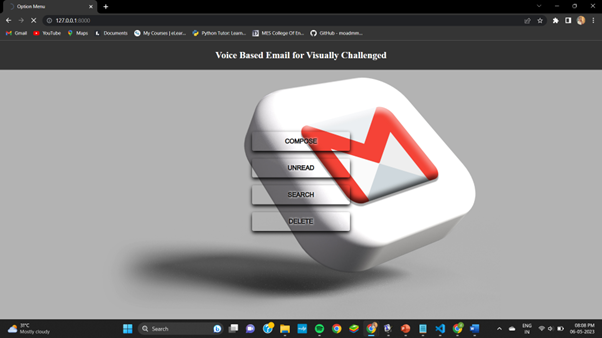
\includegraphics[scale=0.90]{1.png}
  \caption{User Interface 1} 
   \label{fig:is}
\end{center}
\end{figure}
\begin{figure}[htbp]
\begin{center}
  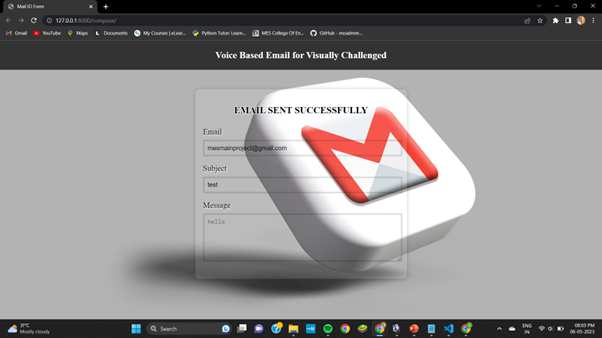
\includegraphics[scale=0.75]{2.png}
  \caption{User Interface 2} 

   \label{fig:is}
\end{center}
\end{figure}
\begin{figure}[htbp]
\begin{center}
  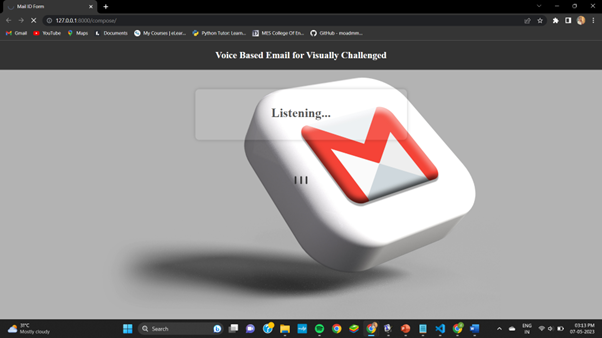
\includegraphics[scale=0.75]{3.png}
  \caption{User Interface 3} 
   \label{fig:is}
\end{center}
\end{figure}
\chapter{Git History}
\begin{figure}[htbp]
\begin{center}
  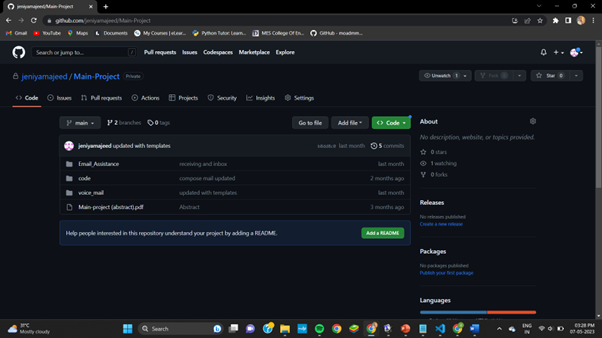
\includegraphics[scale=0.90]{4.png}
  \caption{Git Commits} 
   \label{fig:is}
\end{center}
\end{figure}
\end{document}